% !TEX encoding = UTF-8
% !TEX TS-program = pdflatex
% !TEX root = ../tesi.tex

\chapter{Svolgimento del progetto}
\section{Modello di sviluppo}
	
	Il modello di sviluppo che ho utilizzanto durante lo svolgimento del progetto è il modello iterativo. Questo modello prevede un'esecuzione ciclica di:
	\begin{itemize}
		\item Analisi.
		\item Progettazione.
		\item Produzione di prototipi.
		\item Test.
		\item Raffinamento dei prototipi.
	\end{itemize}
	
	\begin{figure}[H]
		\centering
		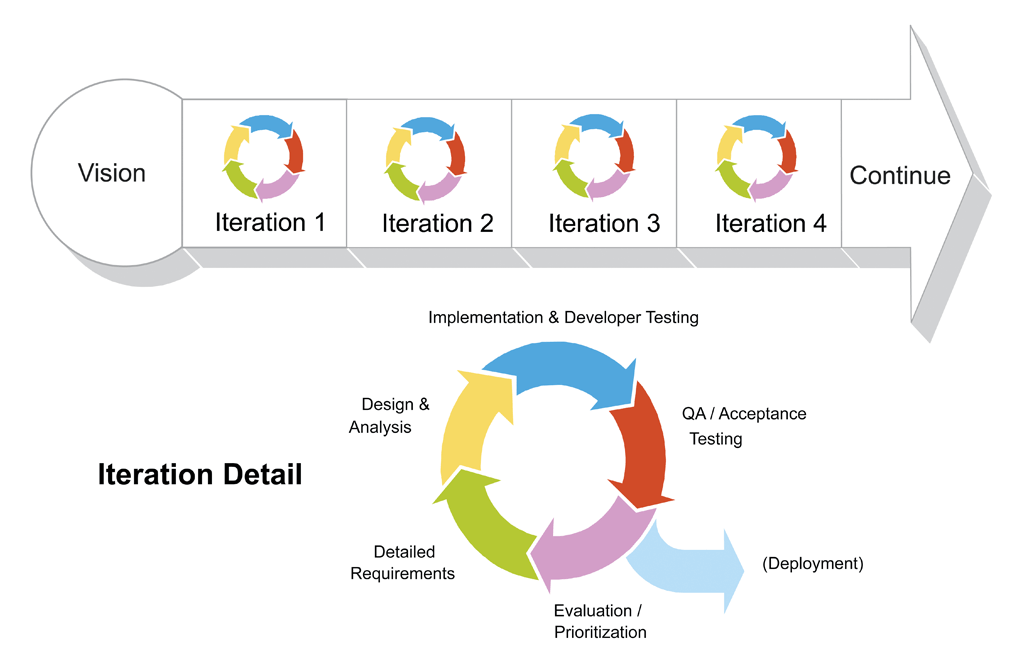
\includegraphics[scale=0.35]{immagini/modello-iterativo}
		\caption{Modello iterativo (\url{https://goo.gl/YcTb7w}).}
	\end{figure}

%	Non posso dire di avere utilizzato il modello incrementale in quanto non ho fissato completamente i requisiti e le funzionalità da implementare all'inizio, ma li ho via via ampliati per meglio accomodare le richieste del \textit{tutor}.
%	Inoltre, ho proceduto con l'implementazione dei \textit{test} automatici solamente nell'ultimo periodo del progetto. Un incremento prevede, oltre all'esecuzione di \textit{test} di unità e integrazione, anche la validazione dell'intero sistema prima di passare allo sviluppo dell'incremento successivo. 
	
	Il principale rischio del procedere per iterazioni piuttosto che per \gls{incrementi} è quello di non convergere mai ad una soluzione. Ho quindi adottato delle soluzioni per ridurre questo rischio: 
	\begin{itemize}
		\item La prima soluzione è stata fissare con il \textit{tutor} un insieme minimo di requisiti obbligatori da implementare nel prodotto, in modo da avere una soluzione accettabile in un periodo relativamente poco avanzato del progetto.
		\item La seconda soluzione è stato l'impiego di prototipi da presentare durante gli incontri con il tutor per dare una migliore idea del prodotto in corso di realizzazione.
	\end{itemize}

	Il procedere per prototipi, oltre ad essere utilizzato ampiamente in IBC, è un metodo che si è rivelato efficace anche nel mio caso. Infatti un prototipo, rispetto alla sola documentazione: 
	\begin{itemize}
		\item Fornisce una migliore visione d'insieme del prodotto, garantendo maggiore comprensibilità anche da parte del personale non tecnico.
		\item Richiede relativamente poco tempo per essere prodotto e modificato, permettendo maggiore flessibilità nel caso di modifiche. Inoltre, diminuisce di molto il tempo che intercorre tra il momento della decisione della modifica e la presentazione del prototipo successivo che la implementa.
		\item Permette di comprendere meglio anche il \textit{design} grafico e l'esperienza di utilizzo volute dal committente nei periodi iniziali del progetto.
	\end{itemize}
	Nei primi periodi i prototipi da me prodotti hanno avuto forma cartacea, per poi evolversi in pagine \textit{web} appena ho preso dimestichezza con Wicket.
	
\section{Analisi dei requisiti}
	Dopo aver completato lo studio di fattibilità e scelto tutte le tecnologie necessarie, ho proceduto a effettuare l'analisi dei requisiti.
	
	La metodologia di conduzione dell'analisi che ho utilizzato si è basata principalmente su interviste al \textit{tutor} in modo da identificare innanzitutto i casi d'uso e successivamente i requisiti.
	
	Periodicamente ho effettuato incontri con il \textit{tutor} per verificare la corretta comprensione dei requisiti. In questo modo, nonostante io non abbia prodotto documentazione formale sull'analisi, ho ridotto il rischio di incomprensioni difficili da correggere se mantenute durante tutta la durata del processo di sviluppo.
	
	Inoltre, per ridurre ulteriormente il rischio di implementare funzionalità non volute o in modo errato, ho prodotto quasi fin da subito dei prototipi da presentare durante gli incontri, come esposto nella sezione precedente.
	
	\subsection{Scopo del prodotto}
		L'applicazione prodotta doveva essere una \textit{web app} che permettesse all'utente di inserire, visualizzare, modificare e rimuovere prodotti commerciali di varie tipologie. L'applicazione doveva considerare categorie e sottocategorie di prodotti. Ad esempio, la pasta è una sottocategorie dei prodotti alimentari.
		
		Per ogni prodotto, l'utente doveva essere in grado di inserire le informazioni, obbligatorie od opzionali, imposte dalla categoria di prodotto. Oltre a queste informazioni, l'utente doveva avere la possibilità di inserire un qualsiasi numero di proprietà aggiuntive non previste dalla tipologia.
		Ogni prodotto poteva avere associata una o più immagini che lo rappresentassero.
		
		Opzionalmente, l'applicazione doveva fornire la possibilità di definire da interfaccia anche nuove tipologie e sottotipologie di prodotto.
	
	\subsection{Attori}
		Il primo passo che ho svolto è stato l'identificazione degli attori. Dato che il \textit{tutor} non ha richiesto l'implementazione di gerarchie di utenti o dell'autenticazione, ho identificato solamente un attore, che d'ora in poi chiamerò \jquote{Utente}.
		
		\begin{figure}[H]
			\centering
			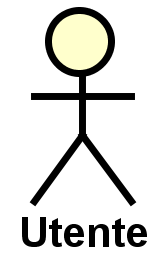
\includegraphics[scale=0.5]{immagini/utente}
			\caption{Attore utente.}
		\end{figure}
		
	\subsection{Casi d'uso}
		Una volta identificato l'attore, ho proceduto a identificare le azioni che egli intendeva svolgere utilizzando il prodotto. A scopo esemplificativo, in questa sezione rappresento alcuni casi d'uso che ho identificato..
		
%		\begin{figure}[H]
%			\centering
%			\includegraphics[width=\textwidth]{{img/uc0.1}.png}
%			\caption{Panoramica dei casi d'uso - Gestione asset}
%		\end{figure}

		% !TEX encoding = UTF-8
% !TEX TS-program = pdflatex
% !TEX root = ../tesi.tex
{
%\subsection*{Panoramica generale}  
%\begin{figure}[H] 
%	\centering 
%	\includegraphics[scale=0.4]{"immagini/usecase/Panoramica dei casi d'uso"} 
%	\caption{Esempio di casi d'uso.}
%\end{figure}
%\def\arraystretch{1.5}
%\rowcolors{2}{D}{P}
%\begin{tabularx}{\textwidth}{l|p{0.7\textwidth}}
%	\rowcolor{I} \multicolumn{2}{c}{\color{white}\textbf{UC1 - Aggiunta asset}} \\
%	\toprule
%	\endhead
%	\textbf{Attori} & Utente\\
%	\textbf{Descrizione} & l'utente aggiunge un asset\\
%	\textbf{Pre-condizione} & l'utente ha aperto l'applicazione\\
%	\textbf{Post-condizione} & un nuovo asset è stato aggiunto ed è visualizzabile sulla mappa; l'utente visualizza un messaggio che comunica la corretta esecuzione dell'operazione; l'area informativa rimane impostata sull'asset appena inserito; la posizione e il livello di ingrandimento della mappa rimangono invariati\\
%	\textbf{Scenario principale} & \vspace{-1.2em}
%	\begin{enumerate}[leftmargin=*,noitemsep,nosep]
%		\item \nameref{sssec:UC1.1};
%		\item \nameref{sssec:UC1.2};
%		\item \nameref{sssec:UC1.4}.
%	\end{enumerate}\\
%	\textbf{Estensioni} & \vspace{-1.2em}
%	\begin{itemize}[leftmargin=*,noitemsep,nosep]
%		\item \nameref{sssec:UC30}: l’utente interrompe volontariamente l’aggiunta dell’asset
%	\end{itemize}\\
%	\textbf{Scenari alternativi} & \vspace{-1.2em}
%	\begin{itemize}[leftmargin=*,noitemsep,nosep]
%		\item \nameref{sssec:UC1.3};
%		\item \nameref{sssec:UC1.5}.
%	\end{itemize}\\
%	\textbf{Generalizzazioni} &  \\
%	\bottomrule
%\end{tabularx}

\subsection*{UC1 - Visualizzazione lista prodotti}
	\label{sec:UC1}  
	\begin{figure}[H] 
		\centering 
		\includegraphics[scale=0.35]{"immagini/usecase/UC1 - Visualizzazione lista prodotti"} 
		\caption{UC1 - Visualizzazione lista prodotti.}
	\end{figure}
	\def\arraystretch{1.3}
	\rowcolors{2}{D}{P}
	\begin{tabularx}{\textwidth}{l|p{0.7\textwidth}}
%		\caption{UC1 - Visualizzazione lista prodotti}
		\rowcolor{I} \multicolumn{2}{c}{\color{white}\textbf{UC1 - Visualizzazione lista prodotti}} \\
		\toprule
		\endhead
		\textbf{Attori} & Utente.\\
		\textbf{Descrizione} & L'utente visualizza la lista dei prodotti presenti all'interno dell'applicazione.\\
		\textbf{Pre-condizione} & L'utente ha aperto l'applicazione.\\
		\textbf{Post-condizione} & L'utente ha visualizzato la lista dei prodotti presenti all'interno dell'applicazione.\\
		\textbf{Scenario principale} & \vspace{-1.2em}
		\begin{enumerate}[leftmargin=*,noitemsep,nosep]
			\item \nameref{sec:UC1}.
		\end{enumerate}\\
%		\textbf{Estensioni} & \vspace{-1.2em}
%		\begin{itemize}[leftmargin=*,noitemsep,nosep]
%			\item \nameref{sssec:UC30}: l’utente interrompe volontariamente l’aggiunta dell’asset
%		\end{itemize}\\
%		\textbf{Scenari alternativi} & \vspace{-1.2em}
%		\begin{itemize}[leftmargin=*,noitemsep,nosep]
%			\item \nameref{sssec:UC1.3};
%			\item \nameref{sssec:UC1.5}.
%		\end{itemize}\\
%		\textbf{Generalizzazioni} &  \\
%		\bottomrule
	\end{tabularx}

%\subsection*{UC2 - Visualizzazione dettaglio prodotto}
%	\label{sec:UC2}  
%	\begin{figure}[H] 
%		\centering 
%		\includegraphics[scale=0.6]{"immagini/usecase/UC2 - Visualizzazione dettaglio prodotto"} 
%		\caption{UC2 - Visualizzazione dettaglio prodotto.}
%	\end{figure}
%	\def\arraystretch{1.5}
%	\rowcolors{2}{D}{P}
%	\begin{tabularx}{\textwidth}{l|p{0.7\textwidth}}
%		\rowcolor{I} \multicolumn{2}{c}{\color{white}\textbf{UC2 - Visualizzazione dettaglio prodotto}} \\
%		\toprule
%		\endhead
%		\textbf{Attori} & Utente.\\
%		\textbf{Descrizione} & L'utente visualizza le informazioni di dettaglio di un prodotto.\\
%		\textbf{Pre-condizione} & L'utente ha aperto l'applicazione.\\
%		\textbf{Post-condizione} & L'utente ha visualizzato informazioni di dettaglio di un prodotto.\\
%		\textbf{Scenario principale} & \vspace{-1.2em}
%		\begin{enumerate}[leftmargin=*,noitemsep,nosep]
%			\item \nameref{sec:UC2.1}.
%			\item \nameref{sec:UC2.2}.
%		\end{enumerate}\\
%		%		\textbf{Estensioni} & \vspace{-1.2em}
%		%		\begin{itemize}[leftmargin=*,noitemsep,nosep]
%		%			\item \nameref{sssec:UC30}: l’utente interrompe volontariamente l’aggiunta dell’asset
%		%		\end{itemize}\\
%		%		\textbf{Scenari alternativi} & \vspace{-1.2em}
%		%		\begin{itemize}[leftmargin=*,noitemsep,nosep]
%		%			\item \nameref{sssec:UC1.3};
%		%			\item \nameref{sssec:UC1.5}.
%		%		\end{itemize}\\
%		%		\textbf{Generalizzazioni} &  \\
%		%		\bottomrule
%\end{tabularx}

%\clearpage
%\subsection*{UC2.1 - Visualizzazione nome prodotto}
%\label{sec:UC2.1}  
%%\begin{figure}[H] 
%%	\centering 
%%	\includegraphics[scale=0.6]{"immagini/usecase/UC2 - Visualizzazione dettaglio prodotto"} 
%%	\caption{UC2 - Visualizzazione dettaglio prodotto.}
%%\end{figure}
%\def\arraystretch{1.5}
%\rowcolors{2}{D}{P}
%\begin{tabularx}{\textwidth}{l|p{0.7\textwidth}}
%	\rowcolor{I} \multicolumn{2}{c}{\color{white}\textbf{UC2.1 - Visualizzazione nome prodotto}} \\
%	\toprule
%	\endhead
%	\textbf{Attori} & Utente.\\
%	\textbf{Descrizione} & L'utente visualizza il nome di un prodotto.\\
%	\textbf{Pre-condizione} & L'utente ha aperto l'applicazione.\\
%	\textbf{Post-condizione} & L'utente ha visualizzato il nome di un prodotto.\\
%	\textbf{Scenario principale} & \vspace{-1.2em}
%	\begin{enumerate}[leftmargin=*,noitemsep,nosep]
%		\item \nameref{sec:UC2.1}.
%	\end{enumerate}\\
%	%		\textbf{Estensioni} & \vspace{-1.2em}
%	%		\begin{itemize}[leftmargin=*,noitemsep,nosep]
%	%			\item \nameref{sssec:UC30}: l’utente interrompe volontariamente l’aggiunta dell’asset
%	%		\end{itemize}\\
%	%		\textbf{Scenari alternativi} & \vspace{-1.2em}
%	%		\begin{itemize}[leftmargin=*,noitemsep,nosep]
%	%			\item \nameref{sssec:UC1.3};
%	%			\item \nameref{sssec:UC1.5}.
%	%		\end{itemize}\\
%	%		\textbf{Generalizzazioni} &  \\
%	%		\bottomrule
%\end{tabularx}
%
%\subsection*{UC2.2 - Visualizzazione proprietà prodotto}
%\label{sec:UC2.2}  
%%\begin{figure}[H] 
%%	\centering 
%%	\includegraphics[scale=0.6]{"immagini/usecase/UC2 - Visualizzazione dettaglio prodotto"} 
%%	\caption{UC2 - Visualizzazione dettaglio prodotto.}
%%\end{figure}
%\def\arraystretch{1.5}
%\rowcolors{2}{D}{P}
%\begin{tabularx}{\textwidth}{l|p{0.7\textwidth}}
%	\rowcolor{I} \multicolumn{2}{c}{\color{white}\textbf{UC2.2 - Visualizzazione proprietà prodotto}} \\
%	\toprule
%	\endhead
%	\textbf{Attori} & Utente.\\
%	\textbf{Descrizione} & L'utente visualizza le proprietà di un prodotto.\\
%	\textbf{Pre-condizione} & L'utente ha aperto l'applicazione.\\
%	\textbf{Post-condizione} & L'utente ha visualizzato le proprietà di un prodotto.\\
%	\textbf{Scenario principale} & \vspace{-1.2em}
%	\begin{enumerate}[leftmargin=*,noitemsep,nosep]
%		\item \nameref{sec:UC2.2}.
%	\end{enumerate}\\
%	%		\textbf{Estensioni} & \vspace{-1.2em}
%	%		\begin{itemize}[leftmargin=*,noitemsep,nosep]
%	%			\item \nameref{sssec:UC30}: l’utente interrompe volontariamente l’aggiunta dell’asset
%	%		\end{itemize}\\
%	%		\textbf{Scenari alternativi} & \vspace{-1.2em}
%	%		\begin{itemize}[leftmargin=*,noitemsep,nosep]
%	%			\item \nameref{sssec:UC1.3};
%	%			\item \nameref{sssec:UC1.5}.
%	%		\end{itemize}\\
%	%		\textbf{Generalizzazioni} &  \\
%	%		\bottomrule
%\end{tabularx}
%
%\subsection*{UC3 - Inserimento prodotto}
%\label{sec:UC3}  
%%\begin{figure}[H] 
%%	\centering 
%%	\includegraphics[scale=0.6]{"immagini/usecase/UC3 - Inserimento prodotto"} 
%%	\caption{UC2 - Visualizzazione dettaglio prodotto.}
%%\end{figure}
%\def\arraystretch{1.5}
%\rowcolors{2}{D}{P}
%\begin{tabularx}{\textwidth}{l|p{0.7\textwidth}}
%	\rowcolor{I} \multicolumn{2}{c}{\color{white}\textbf{UC3 - Inserimento prodotto}} \\
%	\toprule
%	\endhead
%	\textbf{Attori} & Utente.\\
%	\textbf{Descrizione} & L'utente inserisce un nuovo prodotto.\\
%	\textbf{Pre-condizione} & L'utente ha aperto l'applicazione.\\
%	\textbf{Post-condizione} & L'utente ha inserito un nuovo prodotto.\\
%	\textbf{Scenario principale} & \vspace{-1.2em}
%	\begin{enumerate}[leftmargin=*,noitemsep,nosep]
%				\item \nameref{sec:UC3}.
%			\end{enumerate}\\
%%	\begin{enumerate}[leftmargin=*,noitemsep,nosep]
%%		\item \nameref{sec:UC3.1}.
%%		\item \nameref{sec:UC3.2}.
%%		\item \nameref{sec:UC3.3}.
%%		\item \nameref{sec:UC3.4}.
%%		\item \nameref{sec:UC3.5}.
%%	\end{enumerate}\\
%
%	%		\textbf{Estensioni} & \vspace{-1.2em}
%	%		\begin{itemize}[leftmargin=*,noitemsep,nosep]
%	%			\item \nameref{sssec:UC30}: l’utente interrompe volontariamente l’aggiunta dell’asset
%	%		\end{itemize}\\
%	%		\textbf{Scenari alternativi} & \vspace{-1.2em}
%	%		\begin{itemize}[leftmargin=*,noitemsep,nosep]
%	%			\item \nameref{sssec:UC1.3};
%	%			\item \nameref{sssec:UC1.5}.
%	%		\end{itemize}\\
%	%		\textbf{Generalizzazioni} &  \\
%	%		\bottomrule
%\end{tabularx}
%
%\subsection*{UC4 - Modifica prodotto}
%\label{sec:UC4}  
%%\begin{figure}[H] 
%%	\centering 
%%	\includegraphics[scale=0.6]{"immagini/usecase/UC2 - Visualizzazione dettaglio prodotto"} 
%%	\caption{UC2 - Visualizzazione dettaglio prodotto.}
%%\end{figure}
%\def\arraystretch{1.5}
%\rowcolors{2}{D}{P}
%\begin{tabularx}{\textwidth}{l|p{0.7\textwidth}}
%	\rowcolor{I} \multicolumn{2}{c}{\color{white}\textbf{UC4 - Modifica prodotto}} \\
%	\toprule
%	\endhead
%	\textbf{Attori} & Utente.\\
%	\textbf{Descrizione} & L'utente modifica le informazioni di un prodotto.\\
%	\textbf{Pre-condizione} & L'utente ha aperto l'applicazione e sta visualizzando le informazioni di un prodotto.\\
%	\textbf{Post-condizione} & L'utente ha modificato le informazioni di un prodotto.\\
%	\textbf{Scenario principale} & \vspace{-1.2em}
%	\begin{enumerate}[leftmargin=*,noitemsep,nosep]
%		\item \nameref{sec:UC4}.
%	\end{enumerate}\\
%	%		\textbf{Estensioni} & \vspace{-1.2em}
%	%		\begin{itemize}[leftmargin=*,noitemsep,nosep]
%	%			\item \nameref{sssec:UC30}: l’utente interrompe volontariamente l’aggiunta dell’asset
%	%		\end{itemize}\\
%	%		\textbf{Scenari alternativi} & \vspace{-1.2em}
%	%		\begin{itemize}[leftmargin=*,noitemsep,nosep]
%	%			\item \nameref{sssec:UC1.3};
%	%			\item \nameref{sssec:UC1.5}.
%	%		\end{itemize}\\
%	%		\textbf{Generalizzazioni} &  \\
%	%		\bottomrule
%\end{tabularx}
%
%\subsection*{UC5 - Eliminazione prodotto}
%\label{sec:UC5}  
%%\begin{figure}[H] 
%%	\centering 
%%	\includegraphics[scale=0.6]{"immagini/usecase/UC2 - Visualizzazione dettaglio prodotto"} 
%%	\caption{UC2 - Visualizzazione dettaglio prodotto.}
%%\end{figure}
%\def\arraystretch{1.5}
%\rowcolors{2}{D}{P}
%\begin{tabularx}{\textwidth}{l|p{0.7\textwidth}}
%	\rowcolor{I} \multicolumn{2}{c}{\color{white}\textbf{UC5 - Eliminazione prodotto}} \\
%	\toprule
%	\endhead
%	\textbf{Attori} & Utente.\\
%	\textbf{Descrizione} & L'utente elimina un prodotto.\\
%	\textbf{Pre-condizione} & L'utente ha aperto l'applicazione e sta visualizzando le informazioni di dettaglio del prodotto.\\
%	\textbf{Post-condizione} & L'utente ha eliminato un prodotto.\\
%	\textbf{Scenario principale} & \vspace{-1.2em}
%	\begin{enumerate}[leftmargin=*,noitemsep,nosep]
%		\item \nameref{sec:UC5}.
%	\end{enumerate}\\
%	%		\textbf{Estensioni} & \vspace{-1.2em}
%	%		\begin{itemize}[leftmargin=*,noitemsep,nosep]
%	%			\item \nameref{sssec:UC30}: l’utente interrompe volontariamente l’aggiunta dell’asset
%	%		\end{itemize}\\
%	%		\textbf{Scenari alternativi} & \vspace{-1.2em}
%	%		\begin{itemize}[leftmargin=*,noitemsep,nosep]
%	%			\item \nameref{sssec:UC1.3};
%	%			\item \nameref{sssec:UC1.5}.
%	%		\end{itemize}\\
%	%		\textbf{Generalizzazioni} &  \\
%	%		\bottomrule
%\end{tabularx}
%
%\subsection*{UC6 - Inserimento nuova tipologia di prodotto}
%\label{sec:UC6}  
%%\begin{figure}[H] 
%%	\centering 
%%	\includegraphics[scale=0.6]{"immagini/usecase/UC2 - Visualizzazione dettaglio prodotto"} 
%%	\caption{UC2 - Visualizzazione dettaglio prodotto.}
%%\end{figure}
%\def\arraystretch{1.5}
%\rowcolors{2}{D}{P}
%\begin{tabularx}{\textwidth}{l|p{0.7\textwidth}}
%	\rowcolor{I} \multicolumn{2}{c}{\color{white}\textbf{UC6 - Inserimento nuova tipologia di prodotto}} \\
%	\toprule
%	\endhead
%	\textbf{Attori} & Utente.\\
%	\textbf{Descrizione} & L'utente inserisce una nuova tipologia di prodotto.\\
%	\textbf{Pre-condizione} & L'utente ha aperto l'applicazione.\\
%	\textbf{Post-condizione} & L'utente ha inserito una nuova tipologia di prodotto.\\
%	\textbf{Scenario principale} & \vspace{-1.2em}
%	\begin{enumerate}[leftmargin=*,noitemsep,nosep]
%		\item \nameref{sec:UC6}.
%	\end{enumerate}\\
%	%		\textbf{Estensioni} & \vspace{-1.2em}
%	%		\begin{itemize}[leftmargin=*,noitemsep,nosep]
%	%			\item \nameref{sssec:UC30}: l’utente interrompe volontariamente l’aggiunta dell’asset
%	%		\end{itemize}\\
%	%		\textbf{Scenari alternativi} & \vspace{-1.2em}
%	%		\begin{itemize}[leftmargin=*,noitemsep,nosep]
%	%			\item \nameref{sssec:UC1.3};
%	%			\item \nameref{sssec:UC1.5}.
%	%		\end{itemize}\\
%	%		\textbf{Generalizzazioni} &  \\
%	%		\bottomrule
%\end{tabularx}
%
%\subsection*{UC7 - Modifica tipologia prodotto}
%\label{sec:UC7}  
%%\begin{figure}[H] 
%%	\centering 
%%	\includegraphics[scale=0.6]{"immagini/usecase/UC2 - Visualizzazione dettaglio prodotto"} 
%%	\caption{UC2 - Visualizzazione dettaglio prodotto.}
%%\end{figure}
%\def\arraystretch{1.5}
%\rowcolors{2}{D}{P}
%\begin{tabularx}{\textwidth}{l|p{0.7\textwidth}}
%	\rowcolor{I} \multicolumn{2}{c}{\color{white}\textbf{UC7 - Modifica tipologia prodotto}} \\
%	\toprule
%	\endhead
%	\textbf{Attori} & Utente.\\
%	\textbf{Descrizione} & L'utente modifica una tipologia di prodotto.\\
%	\textbf{Pre-condizione} & L'utente ha aperto l'applicazione. È presente almeno una tipologia di prodotto all'interno dell'applicazione.\\
%	\textbf{Post-condizione} & L'utente ha modificato una tipologia di prodotto.\\
%	\textbf{Scenario principale} & \vspace{-1.2em}
%	\begin{enumerate}[leftmargin=*,noitemsep,nosep]
%		\item \nameref{sec:UC7}.
%	\end{enumerate}\\
%	%		\textbf{Estensioni} & \vspace{-1.2em}
%	%		\begin{itemize}[leftmargin=*,noitemsep,nosep]
%	%			\item \nameref{sssec:UC30}: l’utente interrompe volontariamente l’aggiunta dell’asset
%	%		\end{itemize}\\
%	%		\textbf{Scenari alternativi} & \vspace{-1.2em}
%	%		\begin{itemize}[leftmargin=*,noitemsep,nosep]
%	%			\item \nameref{sssec:UC1.3};
%	%			\item \nameref{sssec:UC1.5}.
%	%		\end{itemize}\\
%	%		\textbf{Generalizzazioni} &  \\
%	%		\bottomrule
%\end{tabularx}
%
%\subsection*{UC8 - Eliminazione tipologia prodotto}
%\label{sec:UC8}  
%%\begin{figure}[H] 
%%	\centering 
%%	\includegraphics[scale=0.6]{"immagini/usecase/UC2 - Visualizzazione dettaglio prodotto"} 
%%	\caption{UC2 - Visualizzazione dettaglio prodotto.}
%%\end{figure}
%\def\arraystretch{1.5}
%\rowcolors{2}{D}{P}
%\begin{tabularx}{\textwidth}{l|p{0.7\textwidth}}
%	\rowcolor{I} \multicolumn{2}{c}{\color{white}\textbf{UC8 - Eliminazione tipologia prodotto}} \\
%	\toprule
%	\endhead
%	\textbf{Attori} & Utente.\\
%	\textbf{Descrizione} & L'utente elimina una tipologia di prodotto.\\
%	\textbf{Pre-condizione} & L'utente ha aperto l'applicazione. È presente almeno una tipologia di prodotto all'interno dell'applicazione.\\
%	\textbf{Post-condizione} & L'utente ha eliminato una tipologia di prodotto.\\
%	\textbf{Scenario principale} & \vspace{-1.2em}
%	\begin{enumerate}[leftmargin=*,noitemsep,nosep]
%		\item \nameref{sec:UC8}.
%	\end{enumerate}\\
%	%		\textbf{Estensioni} & \vspace{-1.2em}
%	%		\begin{itemize}[leftmargin=*,noitemsep,nosep]
%	%			\item \nameref{sssec:UC30}: l’utente interrompe volontariamente l’aggiunta dell’asset
%	%		\end{itemize}\\
%	%		\textbf{Scenari alternativi} & \vspace{-1.2em}
%	%		\begin{itemize}[leftmargin=*,noitemsep,nosep]
%	%			\item \nameref{sssec:UC1.3};
%	%			\item \nameref{sssec:UC1.5}.
%	%		\end{itemize}\\
%	%		\textbf{Generalizzazioni} &  \\
%	%		\bottomrule
%\end{tabularx}
%
\subsection*{UC2 - Esecuzione ricerca}
\label{sec:UC2}  
\begin{figure}[H] 
	\centering 
	\includegraphics[scale=0.35]{"immagini/usecase/UC2 - Esecuzione ricerca"} 
	\caption{UC2 - Esecuzione ricerca.}
\end{figure}
\def\arraystretch{1.3}
\rowcolors{2}{D}{P}
\begin{tabularx}{\textwidth}{l|p{0.7\textwidth}}
	\rowcolor{I} \multicolumn{2}{c}{\color{white}\textbf{UC2 - Esecuzione ricerca}} \\
	\toprule
	\endhead
	\textbf{Attori} & Utente.\\
	\textbf{Descrizione} & L'utente esegue una ricerca.\\
	\textbf{Pre-condizione} & L'utente ha aperto la schermata di ricerca.\\
	\textbf{Post-condizione} & L'utente ha eseguito la ricerca e ne visualizza i risultati.\\
	\textbf{Scenario principale} & \vspace{-1.2em}
	\begin{enumerate}[leftmargin=*,noitemsep,nosep]
		\item \nameref{sec:UC2}.
	\end{enumerate}\\
	%		\textbf{Estensioni} & \vspace{-1.2em}
	%		\begin{itemize}[leftmargin=*,noitemsep,nosep]
	%			\item \nameref{sssec:UC30}: l’utente interrompe volontariamente l’aggiunta dell’asset
	%		\end{itemize}\\
	%		\textbf{Scenari alternativi} & \vspace{-1.2em}
	%		\begin{itemize}[leftmargin=*,noitemsep,nosep]
	%			\item \nameref{sssec:UC1.3};
	%			\item \nameref{sssec:UC1.5}.
	%		\end{itemize}\\
	%		\textbf{Generalizzazioni} &  \\
	%		\bottomrule
\end{tabularx}
}    
	
	\subsection{Requisiti}
		\label{sec:requisiti}
		Successivamente, dopo aver identificato i casi d'uso, ho provveduto a trasformarli in requisiti elementari che descrivessero le caratteristiche che il prodotto avrebbe dovuto avere.
		
		Rendere elementari i requisiti scendendo ad un basso livello di dettaglio è importante per aumentarne la comprensibilità e garantirne l'atomicità, ovvero fare in modo che essi si riferiscano ad una singola e precisa necessità senza alcuna ambiguità.
		
		Nella tabella di seguito fornisco un elenco di alto livello delle principali funzionalità, ricavate dall'analisi dei requisiti, che l'applicazione doveva offrire. Ad ogni funzionalità è associata una certa importanza (obbligatoria, desiderabile o facoltativa).
%		Ogni requisito è identificato con un codice univoco, secondo la seguente notazione:
%		\begin{center}
%			R[Importanza][Tipologia][Codice]
%		\end{center}
%		L'\textbf{importanza} indica quanto gli \gls{stakeholder} valutano quel requisito. Può assumere i seguenti valori:
%		\begin{itemize}
%			\item \textbf{O:} indica un requisito obbligatorio.
%			\item \textbf{D:} indica un requisito desiderabile.
%			\item \textbf{F:} indica un requisito facoltativo.
%		\end{itemize}
%		La \textbf{tipologia} indica la categoria di appartenenza del requisito. Può assumere uno tra i seguenti valori:
%		\begin{itemize}
%			\item \textbf{F:} indica un requisito funzionale;
%%			\item \textbf{Q:} indica un requisito di qualità;
%%			\item \textbf{P:} indica un requisito prestazionale;
%			\item \textbf{V:} indica un requisito di vincolo.
%		\end{itemize}
%		Il \textbf{codice} è un valore numerico progressivo.
%		
		% !TEX encoding = UTF-8
% !TEX TS-program = pdflatex
% !TEX root = ../tesi.tex

\begin{tabularx}{\textwidth}{|l|l|}
	\hline
	 \textbf{Funzionalità} & \textbf{Importanza} \\
	\hline
	Gestione prodotti & Obbligatoria\\
	\hline
	Gestione immagine prodotto & Desiderabile\\
	\hline
	Gestione categorie prodotti & Facoltativa\\
	\hline
	Gestione catalogo immagini prodotti & Facoltativa\\
	\hline
	\caption{Principali funzionalità ricavate dai requisiti.}
\end{tabularx}  
		

\section{Progettazione}

	Per quanto riguarda la progettazione, ho seguito un approccio \jquote{\textit{meet-in-the-middle}}, ovvero ho utilizzato sia l'approccio \textit{top-down} che \textit{bottom-up}.
	
	Il motivo di questa scelta è dovuto a esperienze passate vissute durante lo svolgimento del progetto di \gls{swe}. Infatti, io e il mio \textit{team} avevamo progettato in modo puramente \textit{top-down} senza avere una conoscenza profonda delle tecnologie utilizzate. La conseguenza è stata una progettazione che impiegava \textit{design pattern} non adatti alle tecnologie, la quale ha causato ritardi dovuti alla riprogettazione necessaria a risolvere gli errori.
	
	Per non ripetere lo stesso errore, sono arrivato anche a progettare e codificare alcune componenti di basso livello prima di fissare completamente l'intera architettura. Questa scelta ha avuto un duplice vantaggio:
	\begin{itemize}
		\item In primo luogo, mi ha permesso di convergere ad una soluzione architetturale funzionante e che si adattava bene alle tecnologie utilizzate.
		\item In secondo luogo, la codifica delle componenti grafiche mi ha permesso di avere dei prototipi in periodi relativamente poco avanzati del progetto, con i vantaggi descritti nelle sezioni precedenti.
	\end{itemize}
	
	L'architettura del prodotto si basa sul \textit{design pattern} \textit{Model-View-Controller}, alla cui base c'è il principio di separazione delle responsabilità. Questa scelta si adatta anche al \textit{framework} Wicket, che effettua già una prima separazione della \textit{View} fornendo pagine HTML statiche da popolare tramite codice Java.
	
	\begin{figure}[H]
		\centering
		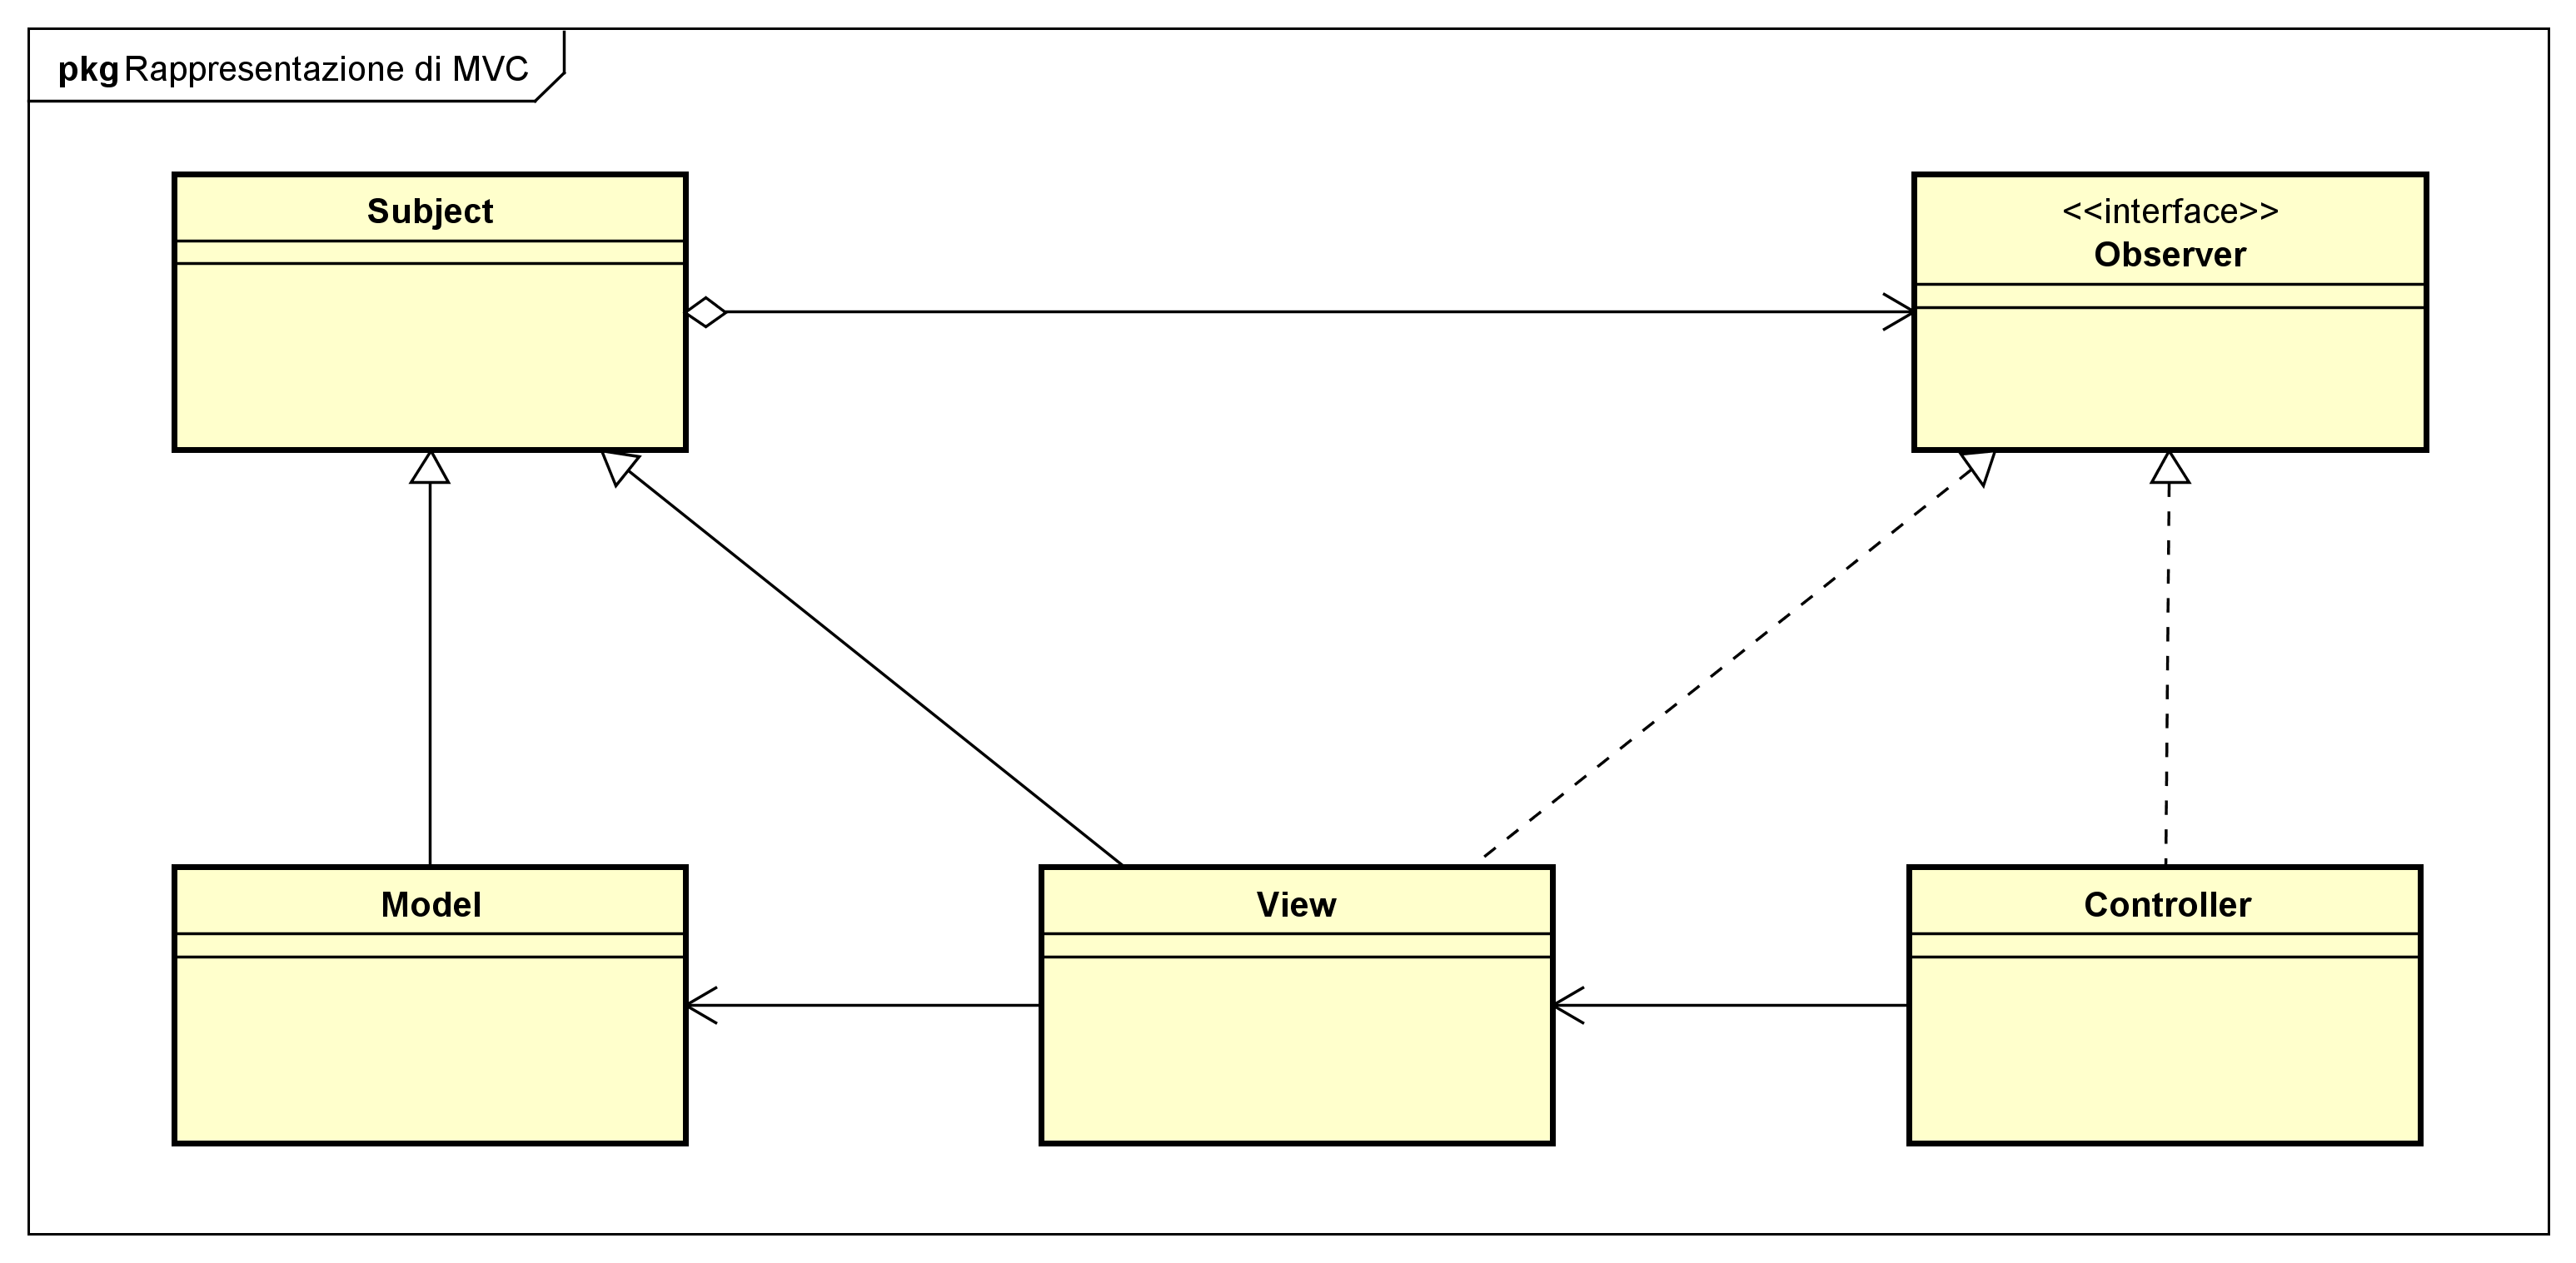
\includegraphics[width=\textwidth]{immagini/mvc}
		\caption{Rappresentazione dell'architettura MVC con \textit{pattern} Observer. (\url{https://goo.gl/NYKkpQ}).}
	\end{figure}

	\subsection{DAO}
		L'accesso ai dati contenuti nel JCR richiede l'utilizzo di API di relativamente basso livello per la lettura e la scrittura. Per separare ulteriormente la logica dell'applicazione da queste API, ho utilizzato il \textit{design pattern} Data Access Object (DAO).
		
		Questo \textit{pattern} consiste nel racchiudere tutte le operazioni che effettuano l'accesso ad un \textit{database} (in questo caso, il JCR) in apposite classi. Gli oggetti di queste classi nascondono l'esistenza di \textit{query} fornendo dei metodi che restituiscono oggetti di \textit{business} utilizzabili direttamente dall'applicazione.
		
		\begin{figure}[H]
			\centering
			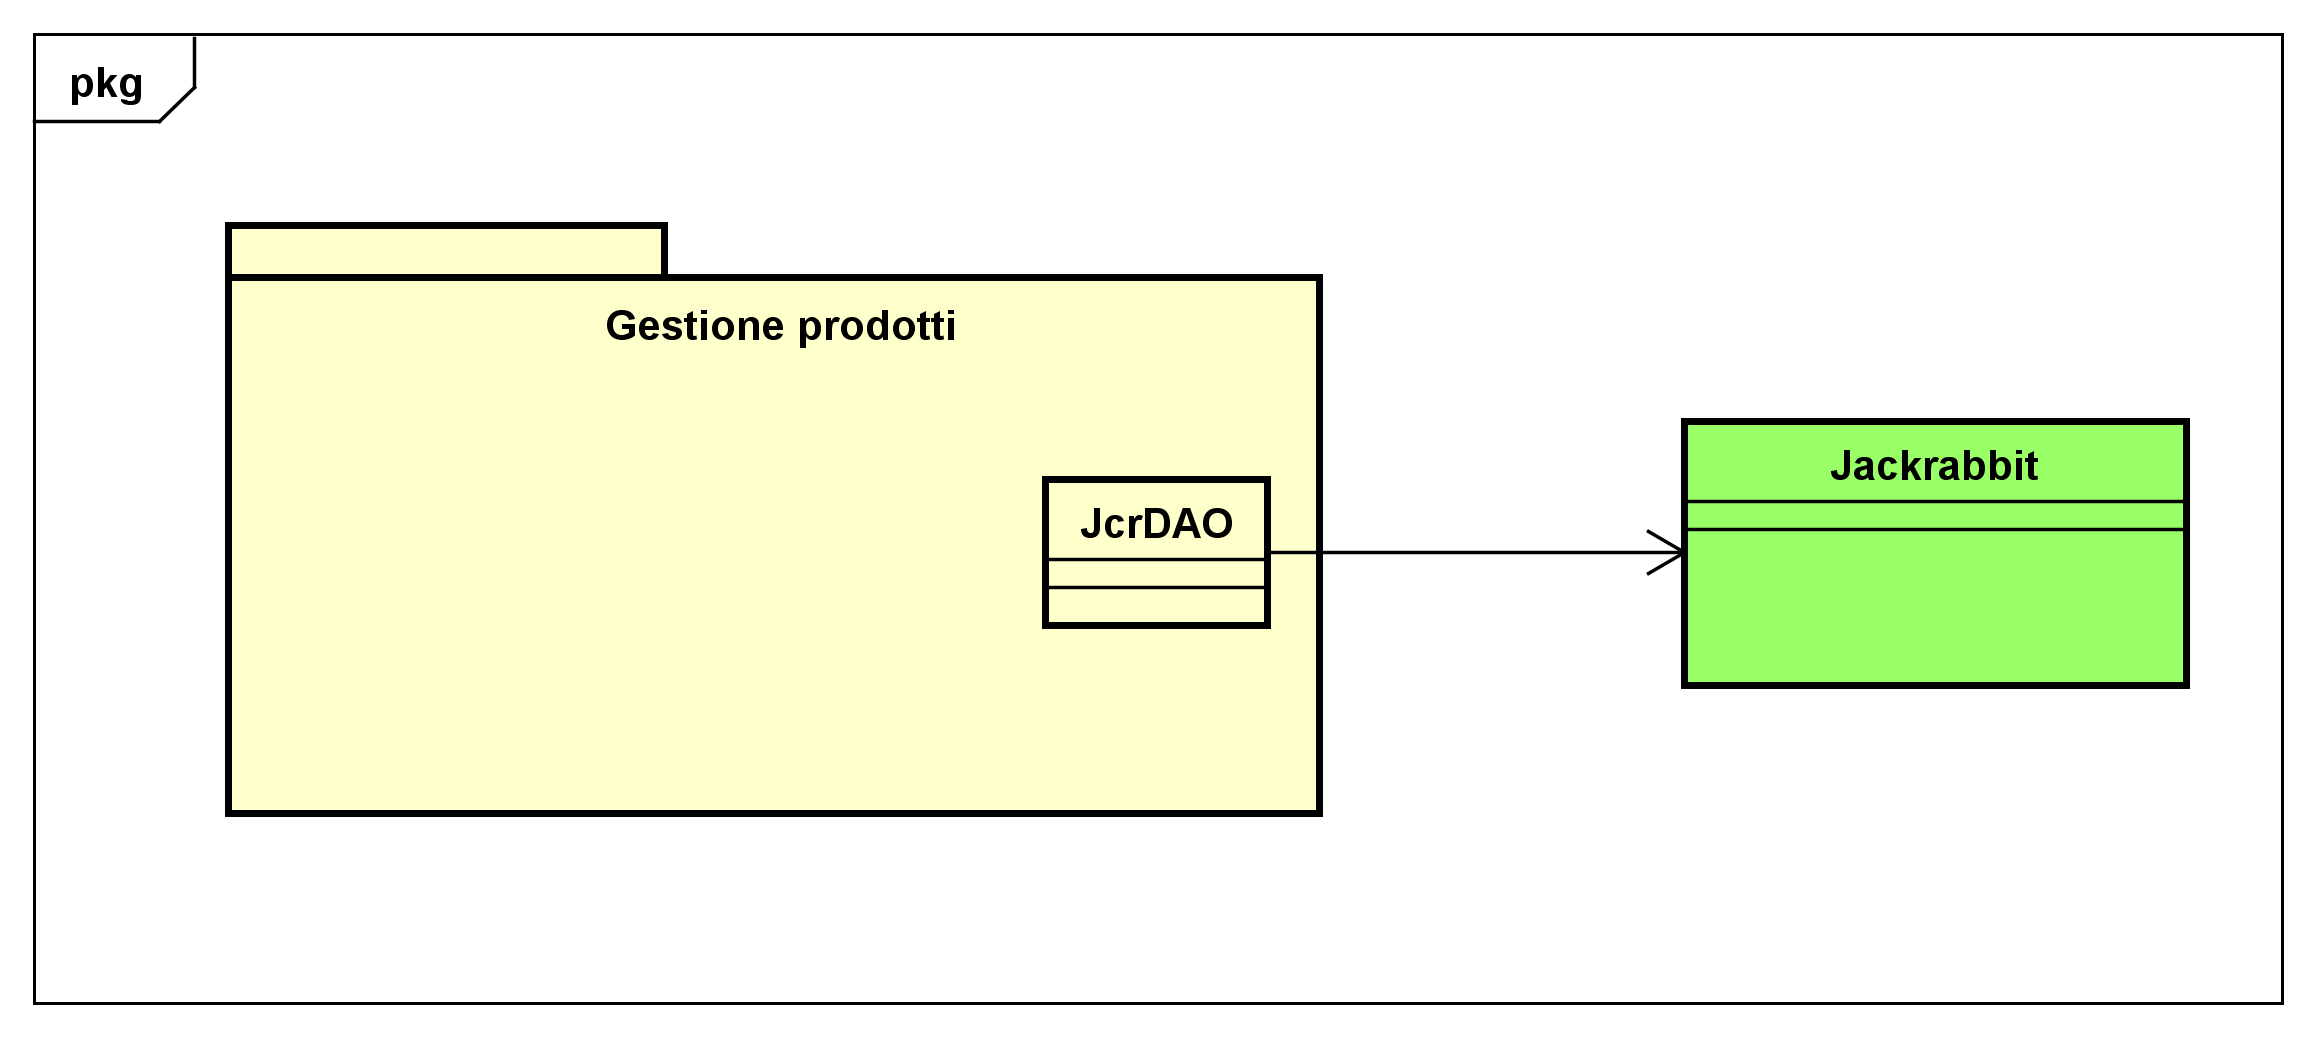
\includegraphics[scale=0.4]{immagini/dao}
			\caption{Ruolo del DAO nell'architettura.}
		\end{figure}
	
	\subsection{Struttura JCR}
		Ho progettato la struttura del contenuto del JCR sotto forma di albero, così come previsto dal modello JCR.
		
		Ogni elemento memorizzato è definito come nodo dell'albero. Ogni nodo può avere delle proprietà e ogni proprietà a sua volta ha un valore. I dati concreti sono memorizzati solamente come valore di una proprietà, le quali diventano quindi le foglie dell'albero.
		
		Includo un esempio minimale di struttura di JCR. Nella rappresentazione, i nodi hanno una forma circolare mentre le proprietà assumono una forma rettangolare.
		
		\begin{figure}[H]
			\centering
			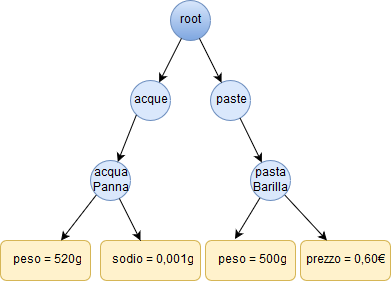
\includegraphics[scale=0.9]{immagini/esempiostrutturajcr}
			\caption{Esempio struttura JCR.}
		\end{figure}
	
	\subsection{\textit{View}}
		Durante la progettazione della \textit{View} ho sfruttato i componenti \texttt{Panel} di Wicket per massimizzare il riuso di codice.
		
		Un \texttt{Panel} infatti può essere utilizzato in diversi punti dell'applicazione senza la necessità di dover ricopiare il \textit{markup} ogni volta. Fornisco un piccolo esempio di progettazione di due pagine diverse che utilizzano lo stesso \texttt{Panel}.
		
		\begin{figure}[H]
			\centering
			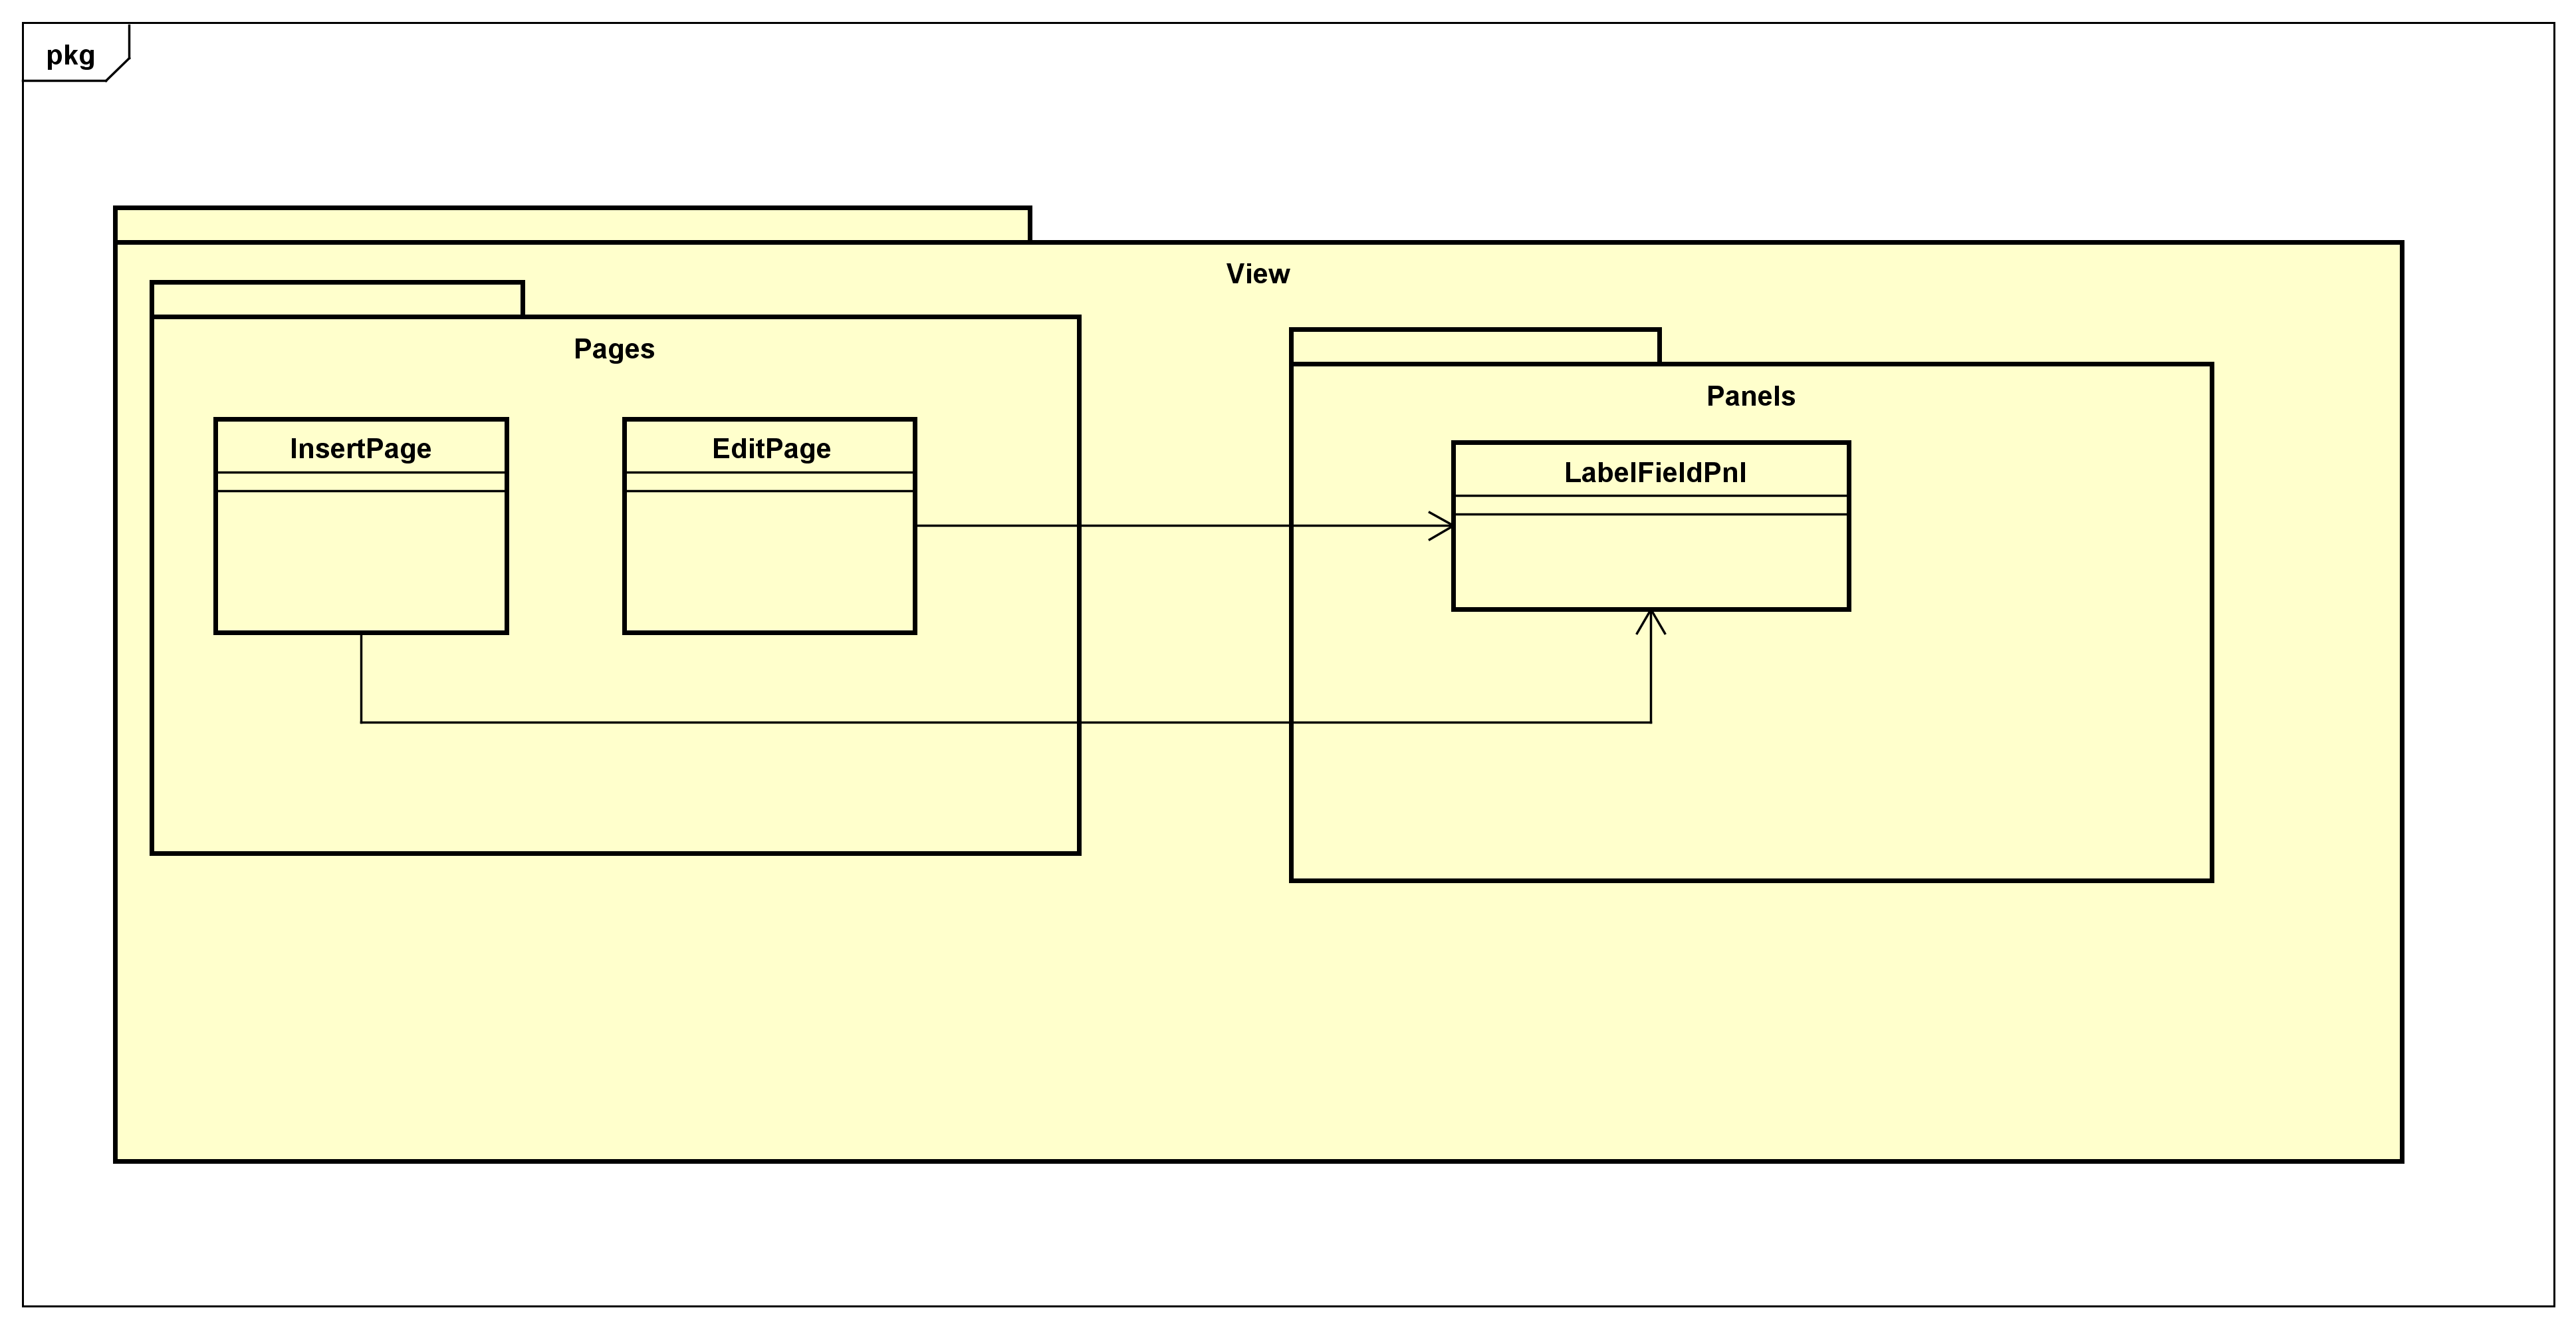
\includegraphics[width=\textwidth]{immagini/pnl}
			\caption{Esempio di utilizzo di \texttt{Panel} di Wicket.}
		\end{figure}
	
		Un altro esempio di utilizzo dei \texttt{Panel} è in combinazione con i componenti \texttt{Repeater}, i quali permettono di creare un componente grafico per ogni elemento presente all'interno di una collezione.
			
\section{Codifica}
	Ho realizzato il prodotto utilizzando i seguenti linguaggi:
	\begin{itemize}
		\item \textbf{Java 8:} per l'utilizzo delle API JCR e la realizzazione della \textit{View} con Wicket.
		\item \textbf{HTML5:} per la creazione del \textit{markup} delle componenti Wicket.
		\item \textbf{CSS:} per assegnare lo stile alle pagine \textit{web}.
		\item \textbf{XML:} per la configurazione di Maven.
		\item \textbf{Compact Namespace and Node Type Definition (CND):} per la definizione dei tipi di nodo e della struttura di JCR. 
	\end{itemize}	
	Nonostante Jackrabbit offrisse API aggiuntive rispetto al JCR, ho utilizzato principalmente quelle specificate dallo \textit{standard} \gls{jsr283}, contenute all'interno di \texttt{javax.jcr.*}. Questa scelta assicura:
	\begin{itemize}
		\item Maggiore compatibilità con altre implementazioni di JCR nel caso di sostituzione della libreria Jackrabbit con un'altra libreria.
		\item Minori problemi in caso di aggiornamento della libreria Jackrabbit, in quanto le API definite dallo \textit{standard} possono cambiare solamente a causa di un aggiornamento dello \textit{standard} stesso. Le API di Jackrabbit invece possono cambiare molto più facilmente e senza preavviso.
	\end{itemize}
	Durante la codifica in Java ho utilizzato alcune caratteristiche del linguaggio che non avevo appreso durante gli studi universitari, tra cui:
	\begin{itemize}
		\item \textbf{Java Annotations:} una forma di metadato da associare ad un qualche elemento del codice in modo da fornire maggiore leggibilità da parte di altri sviluppatori e sopratuttto da parte del compilatore. Alcune delle \textit{annotation} che ho utilizzato maggiormente sono state \texttt{@Override} per la ridefinizione dei metodi e \texttt{@Test} per la specifica dei \textit{test case}.
		\item \textbf{\textit{Reflection}:} meccanismo tramite il quale è possibile ottenere informazioni sul codice e modificare metodi, classi e attributi a \textit{runtime}. La \textit{reflection} viene utilizzata sopratutto da Wicket.
	\end{itemize}
	Per quanto riguarda la rappresentazione degli oggetti di \textit{business}, ho utilizzato dei JavaBean. Questi ultimi sono degli oggetti di classi sottoposte a vari vincoli, tra cui avere solo il costruttore di \textit{default} e permettere l'accesso ai propri campi dati attraverso metodi \texttt{get} e \texttt{set}. Quest'ultimo vincolo, unito alla \textit{reflection}, permette a Wicket di legare i campi dati dei \textit{bean} ai valori dei componenti grafici, in modo da permettere inserimenti e visualizzazioni dei dati.

	Per meglio documentare il codice ho prodotto, attraverso l'utilizzo di Javadoc, una pagina \textit{web} che fornisce descrizioni di classi e metodi.

		
\section{Verifica e validazione}
	Durante tutto lo svolgimento del progetto ho eseguito attività di verifica. Le revisioni periodiche con il \textit{tutor} e i colleghi durante le quali ho dimostrato prototipi, documentazione ed esempi di codice sorgente sono state utili a verificare che il progetto procedesse secondo quanto pianificato. Inoltre, le verifiche sono state utili per la risoluzione dei problemi che ho incontrato durante la codifica.
	
	\subsection{\textit{Test}}
	Un altro tipo di verifica che ho impiegato è quella automatica tramite \textit{test} utilizzando JUnit4. Nonostante io abbia eseguito i \textit{test} di sistema solamente nel periodo finale del progetto, ho effettuato verifiche più mirate tramite \textit{test} di unità nel corso del progetto, sopratutto per quanto riguarda le componenti della \textit{View}. L'utilizzo di \texttt{WicketTester} ha permesso \textit{test} di unità di componenti Wicket senza troppo dispendio di tempo.
	
	Per evitare di dover ridefinire i meccanismi di funzionamento del JCR durante l'esecuzione dei \textit{test} di integrazione, ho utilizzato la classe \texttt{JackrabbitRepositoryStub} fornita da Jackrabbit. Questa classe fornisce uno \gls{stub} di un JCR; l'ho utilizzata per testare l'interazione delle altre componenti con il \textit{repository}.
	
	I \textit{test} di integrazione e di sistema che interagiscono con la \textit{View} sono guidati da un oggetto della classe \texttt{WicketTester}, che permette la simulazione di eventi come l'inserimento di caratteri da tastiera o la pressione di un bottone.
	
	Una delle difficoltà principali che ho incontrato durante l'esecuzione dei \textit{test} di sistema è stata l'interazione tra eventi Ajax e l'invio di \textit{form}. \texttt{WicketTester} infatti fornisce un oggetto di tipo \texttt{FormTester}, che permette l'impostazione di valori degli oggetti contenuti in una data \textit{form} e il successivo invio della stessa. Data la mia inesperienza con gli eventi Ajax, ho impiegato un po' di tempo durante il periodo finale del progetto per capirne il funzionamento e completare i \textit{test} in maniera corretta. Anche grazie all'aiuto della \textit{mailing list} di Wicket, sono riuscito a risolvere i problemi incontrati e ad implementare la maggior parte dei \textit{test} previsti. 
%	Fornisco un elenco dei \textit{test} di sistema pianificati ed eseguiti, utilizzando le seguenti abbreviazioni:
%	\begin{itemize}
%		\item \textbf{NI:} non implementato.
%		\item \textbf{I:} implementato.
%		\item \textbf{NS:} non superato.
%		\item \textbf{S:} superato.
%	\end{itemize}
%	
%	% !TEX encoding = UTF-8
% !TEX TS-program = pdflatex
% !TEX root = ../tesi.tex
{
	\def\arraystretch{1.5}
	\rowcolors{2}{D}{P}
	\begin{longtable}{p{1.5cm}!{\VRule[1pt]}p{5cm}!{\VRule[1pt]}p{1cm}!{\VRule[1pt]}p{1cm}}
		\rowcolor{I}
		\color{white} \textbf{Test} & \color{white} \textbf{Descrizione} & \color{white} \textbf{Stato} & \color{white} \textbf{Esito} \\ 
		\endfirsthead 
		\rowcolor{I} 
		\color{white} \textbf{Test} & \color{white} \textbf{Descrizione} & \color{white} \textbf{Stato} & \color{white} \textbf{Esito} \\ 
		\endhead 
		TS1 & Viene verificato che il sistema permetta la visualizzazione dei prodotti. & \impl & \super \\ 
		TS2 & Viene verificato che il sistema permetta l'inserimento di un prodotto. & \impl & \super \\
		TS3 & Viene verificato che il sistema permetta la modifica di un prodotto. & \impl & \super \\
		TS4 & Viene verificato che il sistema permetta l'eliminazione di un prodotto. & \impl & \super \\
		TS5 & Viene verificato che il sistema permetta l'esecuzione di una ricerca. & \impl & \super \\
		TS6 & Viene verificato che il sistema permetta la visualizzazione dei risultati di una ricerca & \impl & \super \\ 
		TS7 & Viene verificato che il sistema permetta l'associazione di un'immagine ad un prodotto. & \impl & \super \\ 
		TS8 & Viene verificato che il sistema permetta l'associazione di un catalogo di immagini ad un prodotto. & \nonimpl & \nonsuper \\
		TS9 & Viene verificato che il sistema permetta l'inserimento di una nuova tipologia di prodotto. & \nonimpl & \nonsuper \\
		\caption{Test di sistema.}
	\end{longtable}
}  
%	

	Grazie al \textit{plug-in} EclEmma per Eclipse ho potuto calcolare i gradi di copertura del codice da parte dei \textit{test}. Complessivamente, \textit{test} di unità, integrazione e sistema hanno dato i seguenti risultati:
	\begin{table}[H]
		\centering
		\begin{tabular}{|c|c|}
			\hline
			\textbf{Tipo di \textit{coverage}} & \textbf{Percentuale} \\
			\hline
			\gls{statementcoverage} & 85\% \\
			\hline
			\gls{branchcoverage} & 80\%\\
			\hline
		\end{tabular}
		\caption{Resoconto copertura del codice.}
	\end{table}
	Durante la pianificazione e l'implementazione dei \textit{test} ho preferito testare più profondamente le funzionalità di maggior importanza e a maggior rischio di errore, dati anche i vincoli temporali dello \textit{stage}. Per questo motivo le percentuali di copertura non raggiungono il 100\%, ma si attestano in ogni caso su risultati accettabili.
	
	\subsubsection{\textit{Test} prestazionali}
	Uno degli obiettivi del prototipo era l'implementazione di ricerche \textit{full-text} tra gli elementi inseriti. Il \textit{tutor} si è dimostrato interessato alla valutazione prestazionale delle due tipologie di ricerca offerte da JCR:
	\begin{itemize}
		\item La ricerca \jquote{classica}, ovvero eseguita tramite operatore \texttt{LIKE}.
		\item La ricerca \textit{full-text} eseguita tramite operatore \texttt{CONTAINS}.
	\end{itemize}
	
	Ho eseguito \textit{test} prestazionali su un insieme di 20.000 prodotti di tipo pasta strutturati nel seguente modo:
	\begin{table}[H]
		\centering
		\begin{tabular}{|c|c|}
			\hline
			\textbf{Nome attributo} & \textbf{Tipo attributo JCR} \\
			\hline
			id & \texttt{String} \\
			\hline
			prezzo & \texttt{Decimal} \\
			\hline
			minutiCottura & \texttt{Long} \\
			\hline
			volume & \texttt{Decimal} \\
			\hline
			marca & \texttt{String} \\
			\hline
		\end{tabular}
		\caption{Descrizione struttura prodotto utilizzato nei \textit{test} prestazionali.}
	\end{table}
	
	Eseguendo per dieci volte \textit{query} equivalenti, ovvero che ritornavano lo stesso insieme di risultati, ho ottenuto i seguenti risultati:
	
	\begin{table}[H]
		\centering
		\begin{tabular}{|c|c|c|c|c|c|c|c|c|c|c|c|}
			\hline
			\textbf{Operatore} & \multicolumn{10}{c|}{\textbf{Tempo di esecuzione (ms)}} & \textbf{Media} \\
			\hline 
			& \multicolumn{10}{c|}{\textbf{Numero \textit{test}}} & \\
			\hline 
			& \textbf{1} & \textbf{2} & \textbf{3} & \textbf{4} & \textbf{5} & \textbf{6} & \textbf{7} & \textbf{8} & \textbf{9} & \textbf{10} & \\
			\hline 
			CONTAINS & 396 & 476 & 528 & 292 & 805 & 687 & 436 & 557 & 418 & 510 & \green{510,50} \\
			\hline 
			LIKE & 503 & 636 & 697 & 432 & 531 & 747 & 807 & 873 & 772 & 651& \red{665,90} \\
			\hline 
		\end{tabular}
		\caption{Resoconto \textit{test} prestazionali.}
	\end{table}
	
	Come dimostrato dai \textit{test}, l'operatore \texttt{CONTAINS} restituisce i risultati impiegando mediamente un tempo minore del 23\% rispetto all'operatore \texttt{LIKE}. Il motivo di questa differenza è dovuta al fatto che Jackrabbit sfrutta il motore di ricerca testuale fornito da Apache Lucene per l'esecuzione delle ricerche \textit{full-text} con l'operatore \texttt{CONTAINS}. Questo motore è conosciuto per la sua velocità in questo tipo di ricerche.
	
	Ho prodotto un documento destinato a IBC che illustra il procedimento utilizzato per effettuare i \textit{test} prestazionali e i risultati ottenuti.
	
	\subsubsection{Validazione}
	
	Ho eseguito attività di validazione durante gli ultimi giorni dello \textit{stage} mostrando il prodotto al \textit{tutor} e dimostrandogli le funzionalità implementate. Grazie ai \textit{test} di sistema che avevo precedentemente eseguito ho potuto portare a termine la validazione in sicurezza, avendo la garanzia che il sistema rispondesse correttamente ai casi d'uso previsti. Complessivamente, la validazione ha avuto esito positivo.

\section{Prodotto finale}
	Il prodotto finale assume la forma di una \textit{web app} \textit{single-page}. Per istruire l'utilizzatore finale all'utilizzo del prodotto ho redatto un manuale utente comprensivo di immagini. 
	
	Procedo a illustrare alcune funzionalità offerte dal prodotto.
	
	\subsection{\textit{Homepage}}
		L'\textit{homepage} presenta una tabella con struttura ad albero tramite la quale è possibile visualizzare le informazioni dei prodotti. Cliccando sul pulsante \jquote{+} è possibile espandere la visualizzazione delle categorie, fino ad arrivare alla visualizzazione dei prodotti desiderati.
		
		\begin{figure}[H]
			\centering
			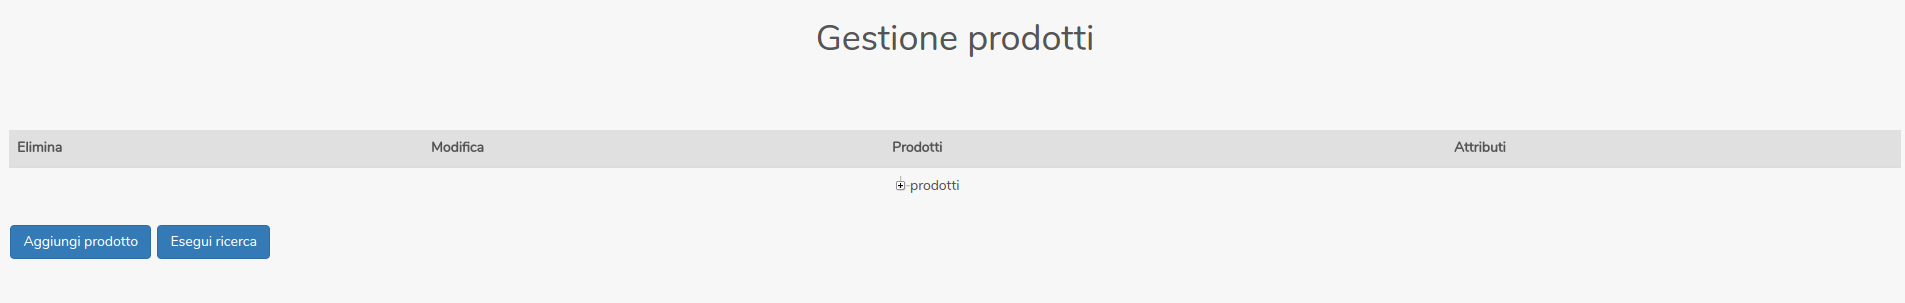
\includegraphics[width=\textwidth]{immagini/home-page-blank}
			\caption{\textit{Homepage} con nessun prodotto visualizzato.}
		\end{figure}
	
		\begin{figure}[H]
			\centering
			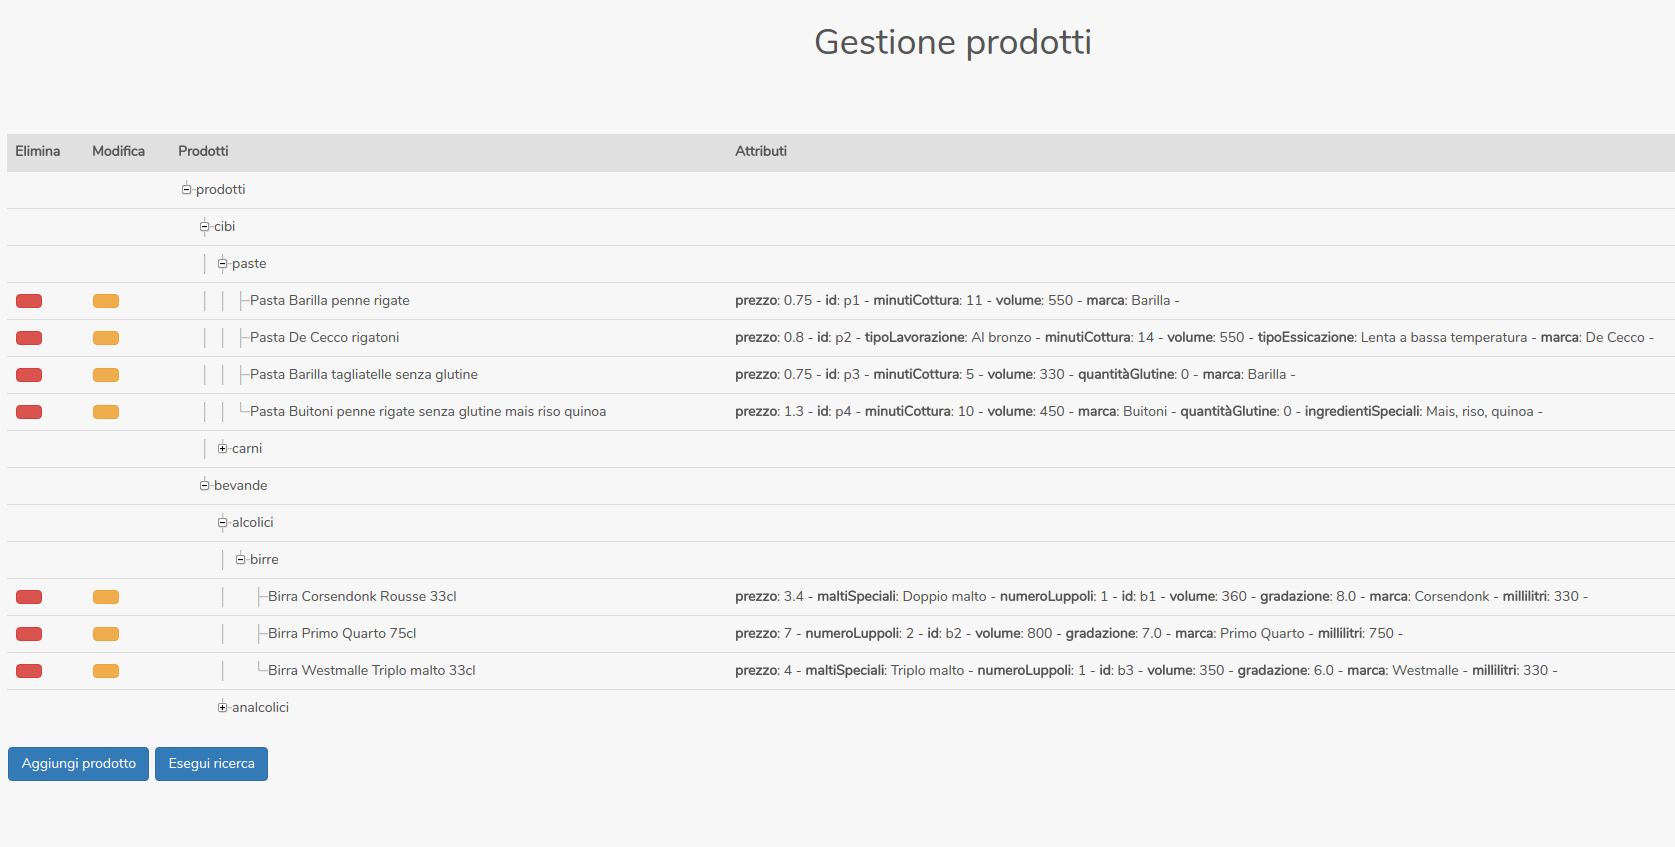
\includegraphics[width=11cm]{immagini/homepage-view-product}
			\caption{\textit{Homepage} con alcuni prodotti visualizzati.}
		\end{figure}
	
	\subsection{Finestra di inserimento}
		La finestra di inserimento permette di aggiungere nuovi prodotti a partire dalle categorie già esistenti. Selezionando la tipologia di prodotto, l'applicazione come prima cosa richiede la compilazione dei campi dati predefiniti. Quelli obbligatori sono segnalati da un asterisco di colore rosso.
		
		Una volta compilati i dati obbligatori, l'utente ha la possibilità di aggiungere proprietà aggiuntive tramite l'utilizzo del pulsante \jquote{Aggiungi riga proprietà}. Una proprietà consiste di tre elementi:
		\begin{itemize}
			\item Un nome.
			\item Un tipo, a scelta fra \texttt{String}, \texttt{Long}, \texttt{Decimal}, \texttt{Double}.
			\item Un valore, in accordo con il tipo scelto.
		\end{itemize}
		Infine, l'utente ha la possibilità di aggiungere una sola immagine da abbinare al prodotto.
		
		\begin{figure}[H]
			\centering
			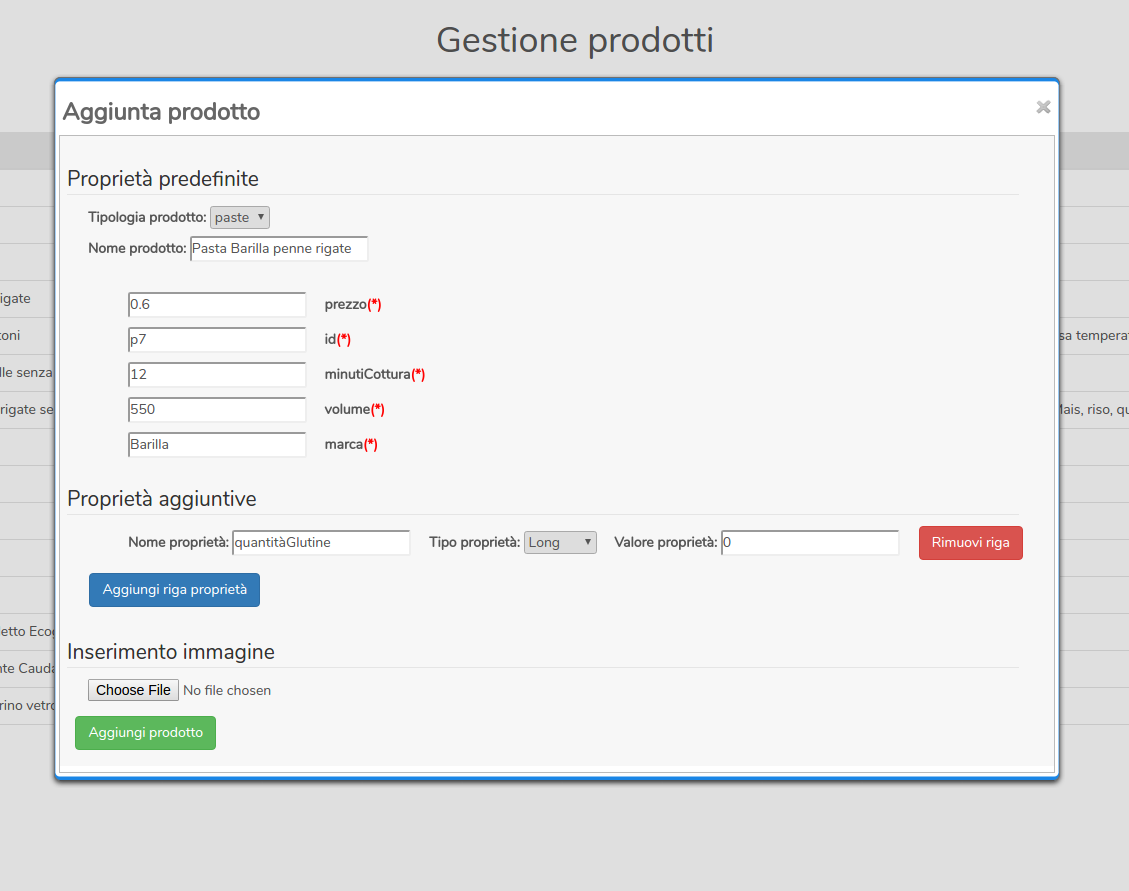
\includegraphics[width=\textwidth]{immagini/add-page}
			\caption{Finestra di inserimento prodotto.}
		\end{figure}
	
	\subsection{Finestra di visualizzazione dettaglio e modifica}
		Cliccando sul pulsante \jquote{Modifica} affianco al nome di un prodotto verrà aperta la finestra di visualizzazione dettaglio e modifica.
		
		All'interno di questa finestra l'utente ha la possibilità di:
		\begin{itemize}
			\item Visualizzare e modificare le informazioni di dettaglio del prodotto.
			\item Rimuovere eventuali proprietà aggiuntive precedentemente inserite. Le proprietà predefinite non possono essere rimosse per non invalidare la struttura imposta dalla categoria del prodotto.
			\item Aggiungere ulteriori proprietà.
			\item Visualizzare e modificare l'immagine che rappresenta il prodotto.
		\end{itemize}
		
		\begin{figure}[H]
			\centering
			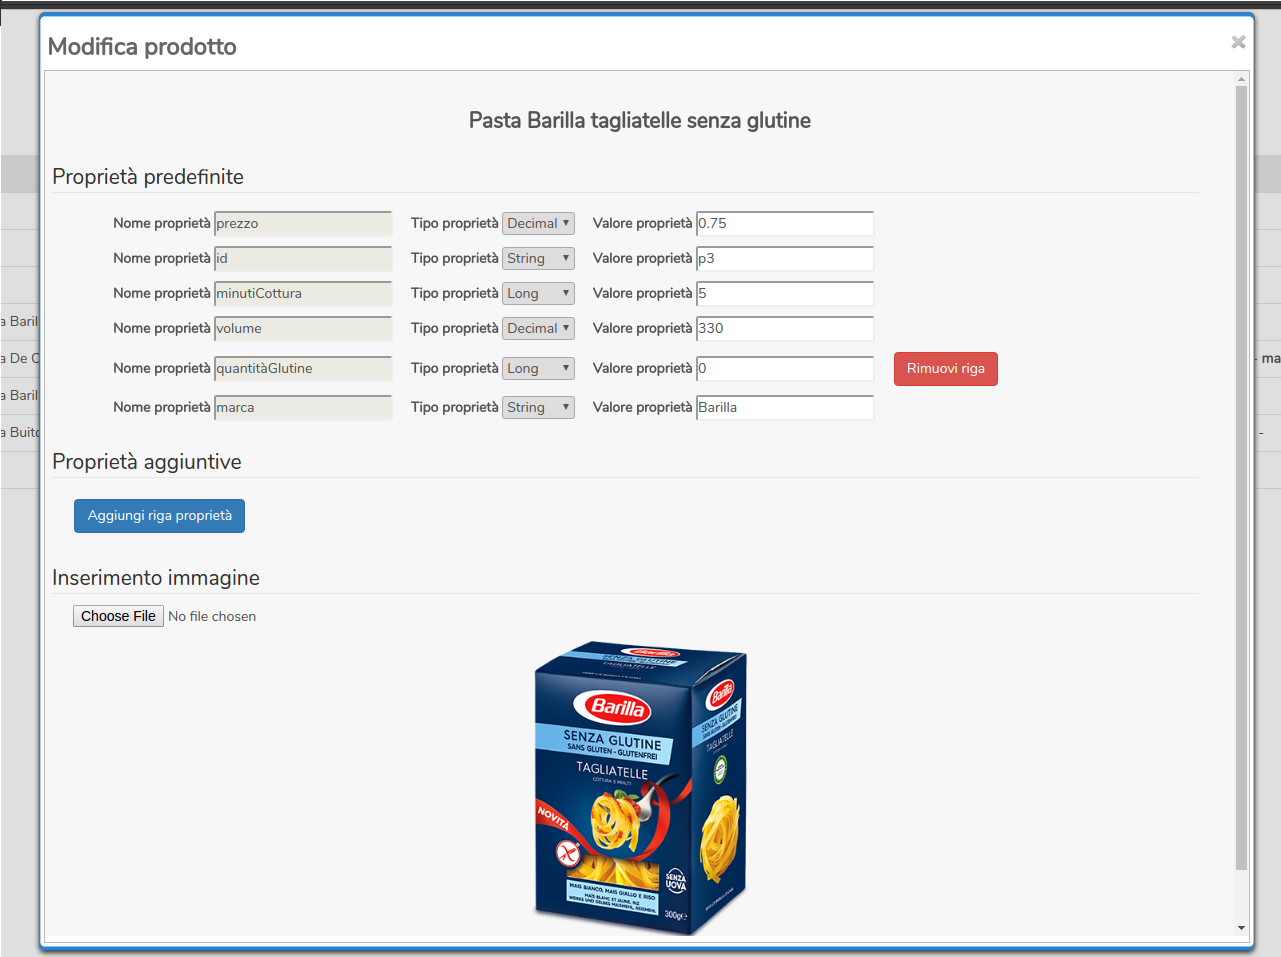
\includegraphics[width=\textwidth]{immagini/edit-page}
			\caption{Finestra di visualizzazione dettaglio e modifica prodotto.}
		\end{figure}
	
	\subsection{Finestra di ricerca}
		Dalla finestra di ricerca l'utente può effettuare ricerche tra i prodotti, raffinando i criteri di selezione fino ad arrivare all'articolo (o all'insieme di articoli) di interesse.
		
		Per effettuare una ricerca è necessario seguire i seguenti passi:
		\begin{itemize}
			\item Come prima cosa, l'applicazione richiede che venga selezionata una tipologia di prodotto su cui fare la ricerca. Le tipologie suggerite sono tutte quelle presenti all'interno del JCR in quel dato momento. Se la tipologia non viene specificata, la ricerca comprenderà i prodotti di tutte le categorie.  
			\item Successivamente, l'utente potrà aggiungere uno o più filtri di ricerca, specificando per ognuno:
				\begin{itemize}
					\item \textbf{Nome della proprietà da ricercare}. L'applicazione suggerisce tutte le proprietà definite dalla struttura della tipologia di prodotto selezionato, più eventuali proprietà aggiuntive.
					\item \textbf{Operatore da applicare}, come ad esempio >, >=, <, <=, =.
					\item \textbf{Valore da ricercare}.
				\end{itemize}	
			\item Una volta eseguita la ricerca, i risultati verranno visualizzati nella stessa finestra. L'utente è libero di modificare e rimuovere i filtri precedentemente utilizzati, oppure di inserirne di nuovi per raffinare la ricerca. 	
		\end{itemize}
		
		\begin{figure}[H]
			\centering
			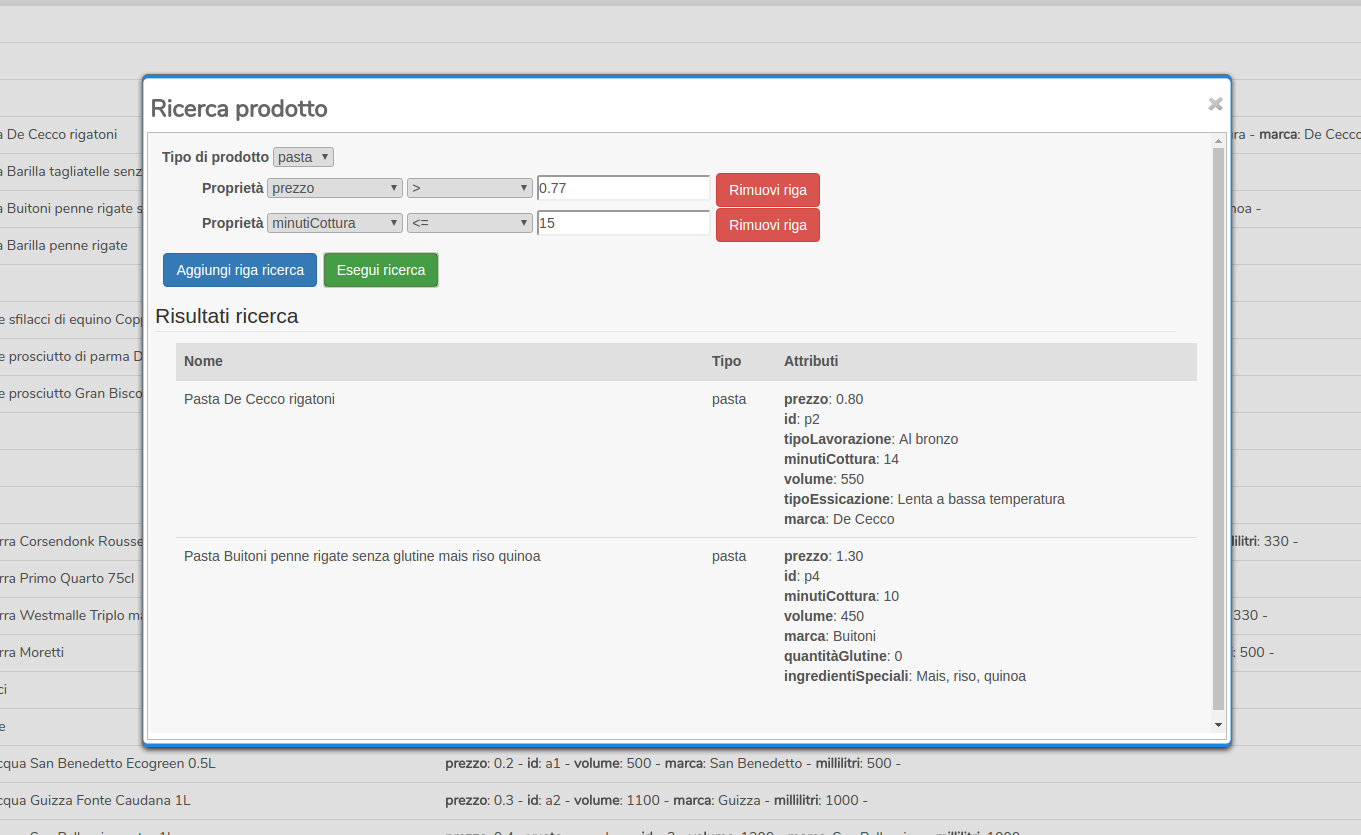
\includegraphics[height=7.1cm, width=\textwidth]{immagini/query-page-doppio}
			\caption{Finestra di ricerca, filtro di selezione multiplo.}
		\end{figure}
	
		Per accedere alla funzionalità di ricerca \textit{full-text}, è sufficiente selezionare la voce \jquote{Tutte} nel \textit{box} che indica la proprietà da ricercare. Così facendo, l'unico operatore disponibile sarà \texttt{CONTAINS}, il quale cercherà il testo immesso dall'utente all'interno di tutte le proprietà di tipo \texttt{String} di tutti i nodi della tipologia specificata.
		
		\begin{figure}[H]
			\centering
			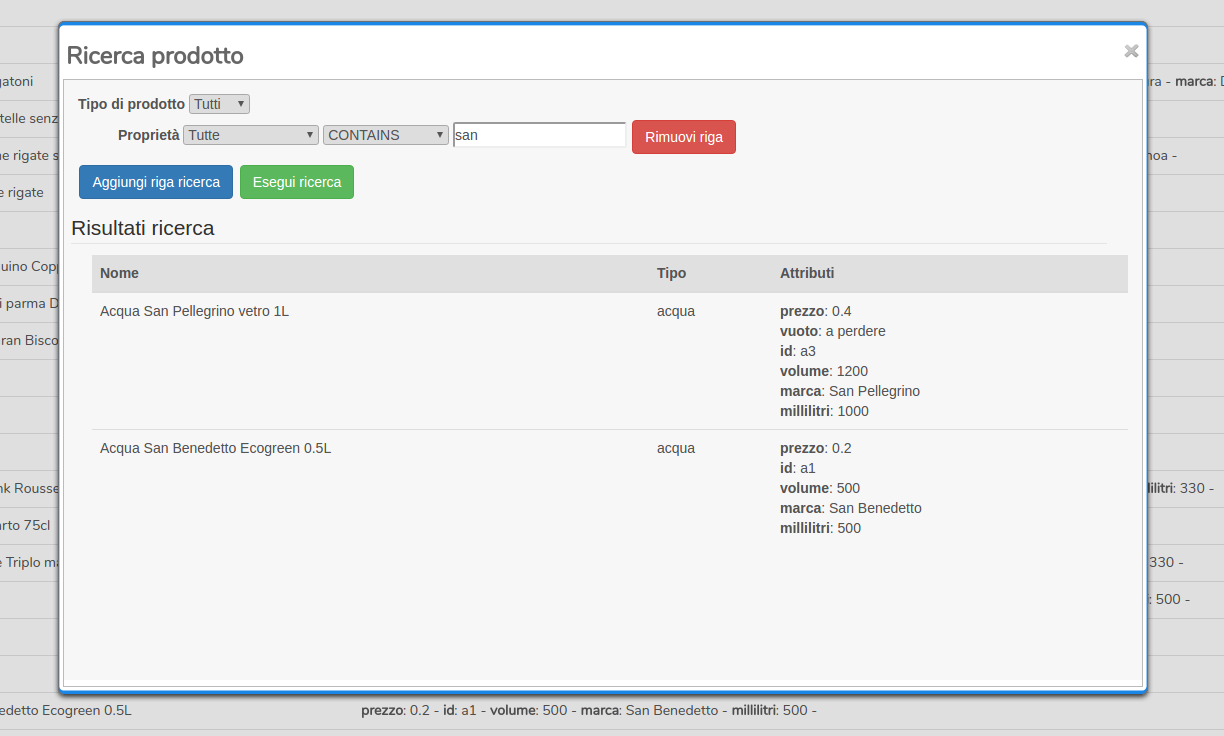
\includegraphics[height=7.1cm, width=\textwidth]{immagini/query-page-contains}
			\caption{Finestra di ricerca, filtro di selezione \textit{full-text}.}
		\end{figure}